

\section{Overview}
This chapter will go through a detailed explanation of each step that should be taken to replicate this software developed for this thesis, starting from nothing more than a Python interpreter. It is important to note that the vast majority of the software development for this project (every change from February onwards) has been documented and explained with comments, descriptions, and a \verb|readme.md| file on a publicly accessible GitHub repository named IPDMP. The link to the Individual Project Data-to-Model Pipeline (IPDMP) repository, as well as an extensive "code walk-through" for each major program discussed can be found in Appendix B. 

\subsection{Section Description}
The methodology for this thesis fundamentally consists of four key steps, which align with the objectives defined in the introduction section. This is a brief overview of the upcoming sections covering brief objective. 
\subsubsection{Objective 1: Image Selection}
\begin{itemize}
    \item Select one appropriate satellite image for the development of the necessary software tools and three more satellite images for model deployment. 
\end{itemize}
The first step is to conduct image download. The two approaches for this application are to either download images locally or use a web-based database such as Google Earth Engine. For this study, locally downloading data is appropriate because there is no need to scale up to a large time period or study area yet. 

\subsubsection{Objective 2: Data Generation}
\begin{itemize}
    \item Develop a software tool to automate satellite imagery handling/pre-processing and facilitate the semi-automated creation of labelled training data through a dedicated user interface. 
\end{itemize}
NALIRA, a Python program, automates the generation of training data from Sentinel 2 imagery, avoiding manual labelling. It processes satellite images by extracting bands, performing cloud masking, calculating indices, and optionally displaying plots. The True Colour Image and index plots are divided into user-defined chunks to simplify labelling. Users are prompted to input the number of reservoirs and water bodies per chunk. If present, a GUI enables users to label these features as Regions of Interest (ROIs), with coordinates saved in a CSV file that undergoes rigorous automated validation. This chunk-wise approach allows for breaks and revisiting previous labels. Finally, the labelled coordinates are used to extract individual reservoir/water body images (and corresponding non-water land images) for training data, sized at $\frac{1}{25}$ of the original chunk.

\subsubsection{Objective 3: Model Training}
\begin{itemize}
    \item Build, train, and validate a machine learning classification model (specifically using the Keras Sequential model) for water reservoirs, non-reservoir water bodies, and land.
\end{itemize}
The third step is to train the machine learning model that will identify reservoirs, water bodies, and land. This is done using a repurposed Google Colab TensorFlow tutorial initially intended for flower classification with a Keras Sequential Model !!! CITE THIS CITE THIS CITE THIS !!!. To repurpose this tutorial, several unnecessary, non-functional, or superfluous steps were removed, reliability was improved by adding robustness to the process, and the original flower classification training data was swapped out for the images generated with NALIRA. The program encompassing the deployment of the model is called the Keras Reservoir Identification Sequencing Platform, abbreviated to KRISP. The program dedicated to the training and initial validation of the final model is called KRISP Trainer. 

\subsubsection{Objective 4: Model Deployment}
\begin{itemize}
    \item Deploy the model over East England and produce a map of the quantity, location, and size of all water reservoirs in East England for March 2025. 
\end{itemize}
The fourth and final step is to deploy the model. For this, the program created is the aforementioned KRISP program. This Python script ingests an un-processed and unseen satellite image from Sentinel 2 then conducts very similar initial steps to NALIRA (image manipulation, cloud masking, index calculation, optional display of the index calculated, optional TCI manipulation, and separation of the full-sized image into chunks smaller chunks). After these steps are complete, KRISP further separates each chunk into 25 "mini-chunks" to match the size of each box containing a training image. This is done to ensure that the test and deployment data for KRISP is the same dimensions as the test upon which KRISP was trained, maximising accuracy and minimising error. 

\section{Objective 1: Image Selection}
\subsection{Satellite Choice}
The satellite of choice for this thesis is Sentinel 2 because of the higher resolution options compared to Landsat 7-9. Additionally, for low-computation troubleshooting, the Sentinel 2 image folders also have a 60m resolution option, reducing time spent on opening and handling the otherwise larger image arrays. 

\subsection{Satellite Compatibility}
While the KRISP trainer program was developed primarily with Sentinel 2 in mind, it is entirely sensor-agnostic, meaning that dependent on specifically Sentinel 2 data. The KRISP trainer program is not only sensor-agnostic, but also 

The NALIRA program was initially developed for Landsat 7 images, then it was adapted for compatibility with any processing level of Landsat 8 and 9 as well. Then, Sentinel 2 data was introduced, and there was a brief period where NALIRA was capable of accepting any image from Landsat 7, Landsat 8, Landsat 9, Sentinel 2A, Sentinel 2B, and Sentinel 2C. 

\subsection{Image Download}
To download images for Sentinel 2, the Copernicus browser must be used. To access these files it is necessary to log in or create an account, which can be done easily by registering a valid email address. 
\begin{figure}[H]
    \centering
    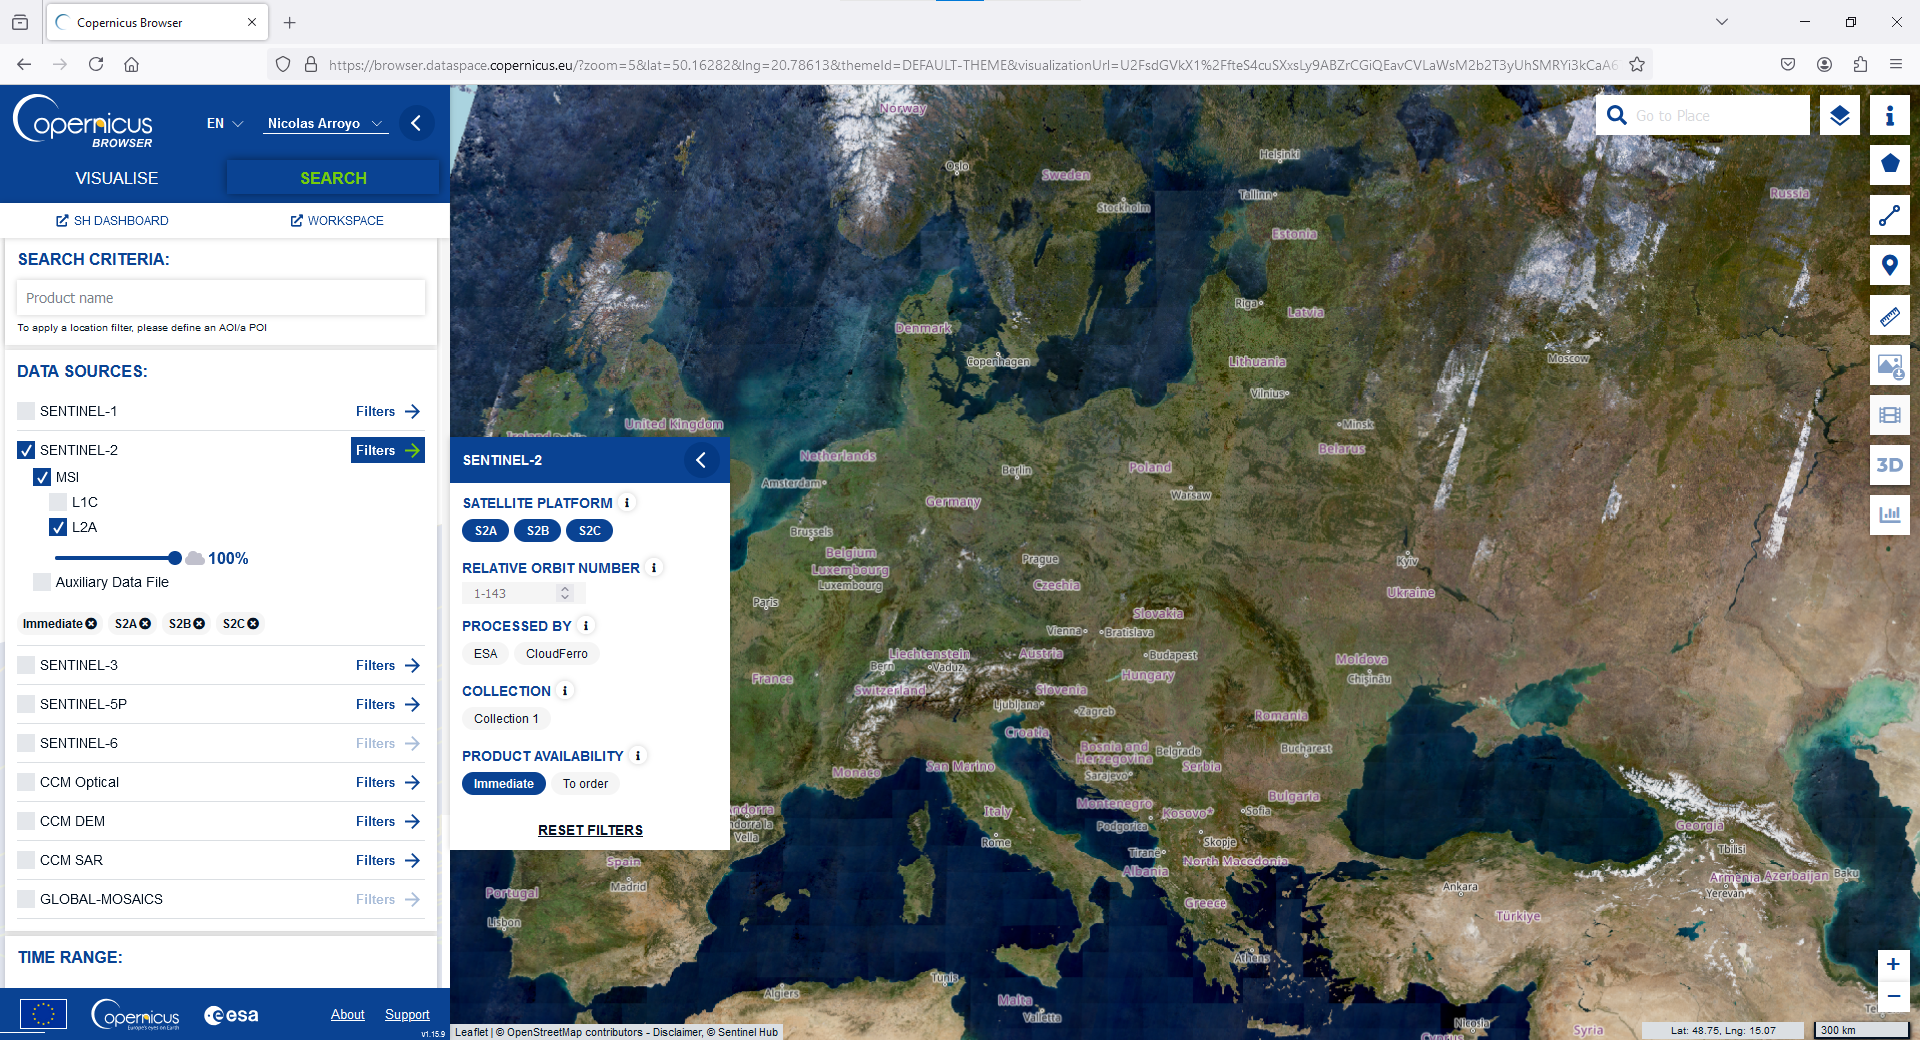
\includegraphics[width=0.5\linewidth]{contents/figures/ME copernicus detailed search.jpg}
    \caption{Copernicus browser detailed search}
    \label{fig:ME copernicus detailed search}
\end{figure}
After logging in or registering an account, the first step of downloading images is to select the appropriate satellite. This thesis focuses on Sentinel 2 images, so we must filter out all other satellites that would not be compatible (figure \ref{fig:ME copernicus detailed search}. Go to "SEARCH" on the upper left and select "SENTINEL 2" $\rightarrow$ "MSI", which stands for Multi-Spectral Instrument. Then, select only "L2A" to filter down the images to the second processing level offered by Sentinel 2. After this, select "Filters" and choose S2A, S2B, and S2C platforms to allow for images from any of the three satellites in the Sentinel constellation.

\begin{figure}[H]
    \centering
    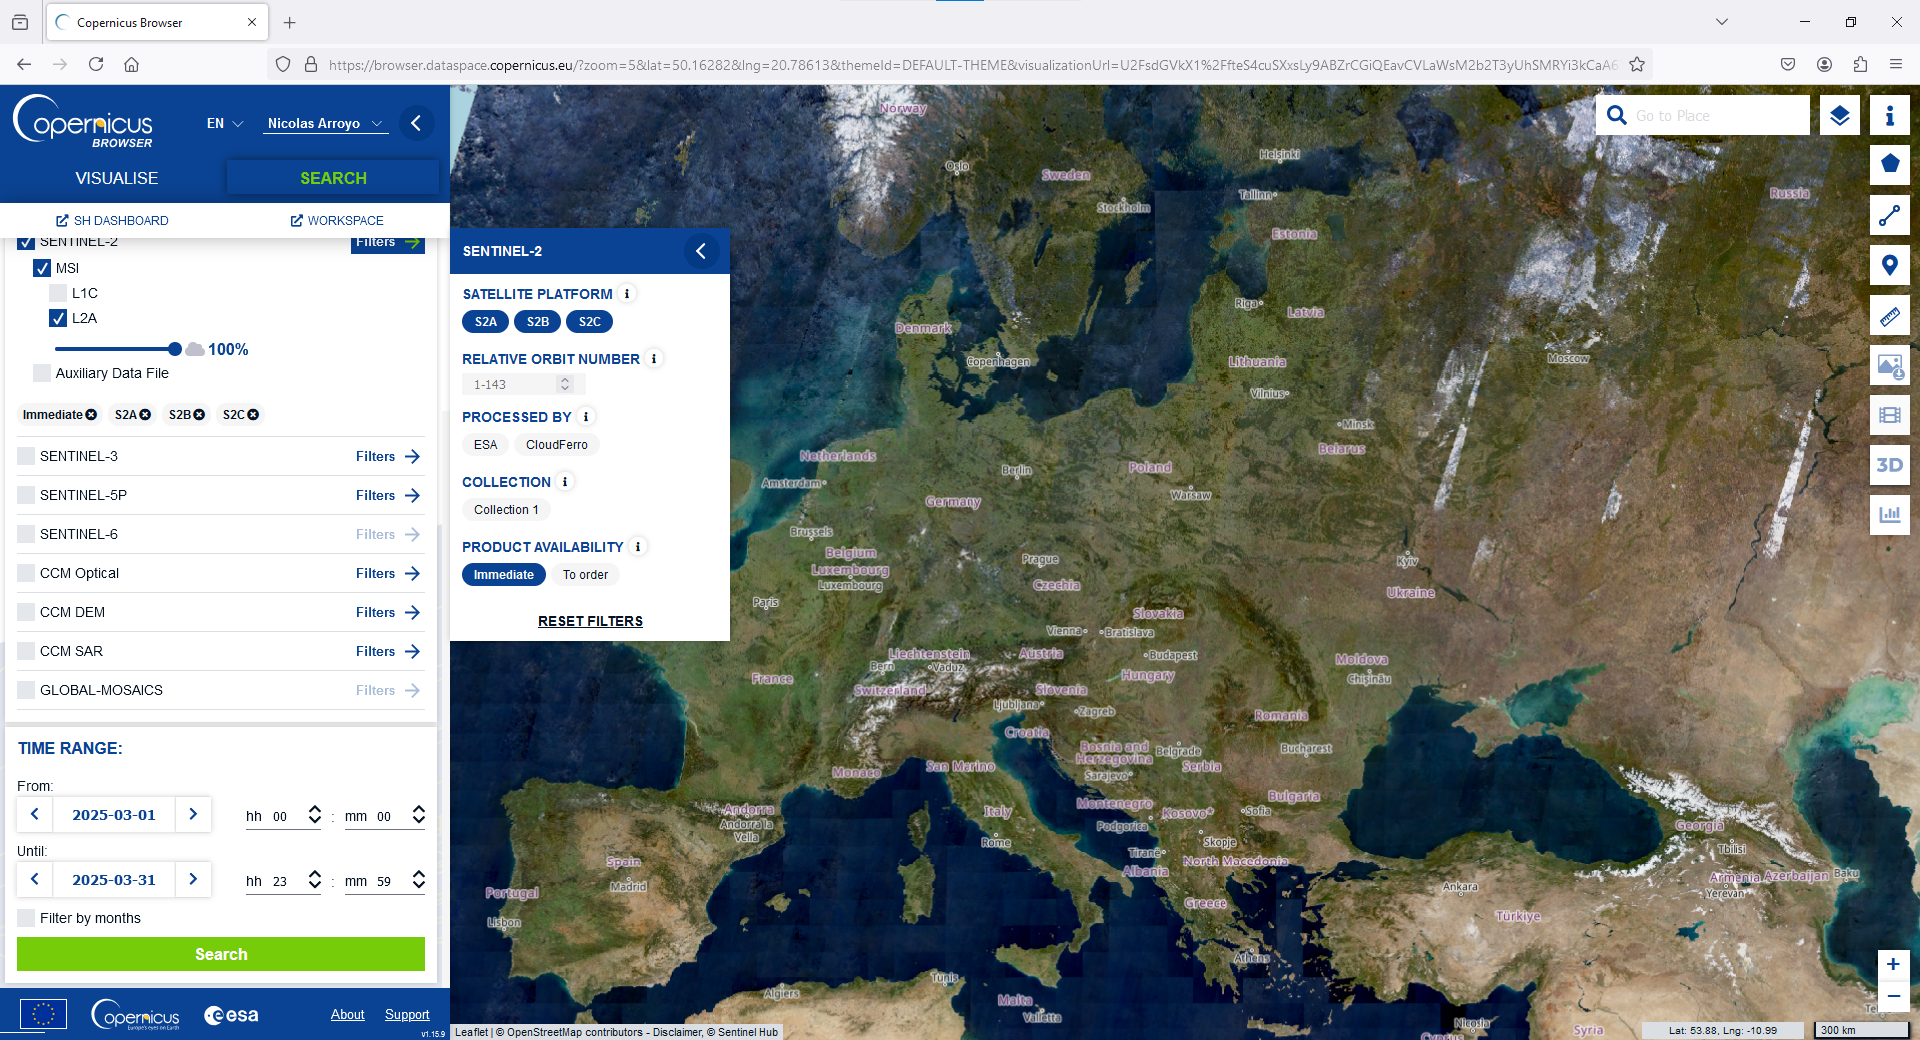
\includegraphics[width=0.5\linewidth]{contents/figures/ME copernicus time range.jpg}
    \caption{Copernicus browser time range example}
    \label{fig:ME copernicus time range}
\end{figure}
Once the satellite platform has been selected, scroll down on the sidebar to reach the time frame of the image (figure \ref{fig:ME copernicus time range}. The time period for this study is the month of March 2025, as was discussed in the introduction, so select "2025-03-01" in the "From:" field and "2025-03-31" in the "Until:" field to encompass this period. Once both time period and satellite platform have been defined, press the green "Search" button at the bottom. 

\begin{figure}[H]
    \centering
    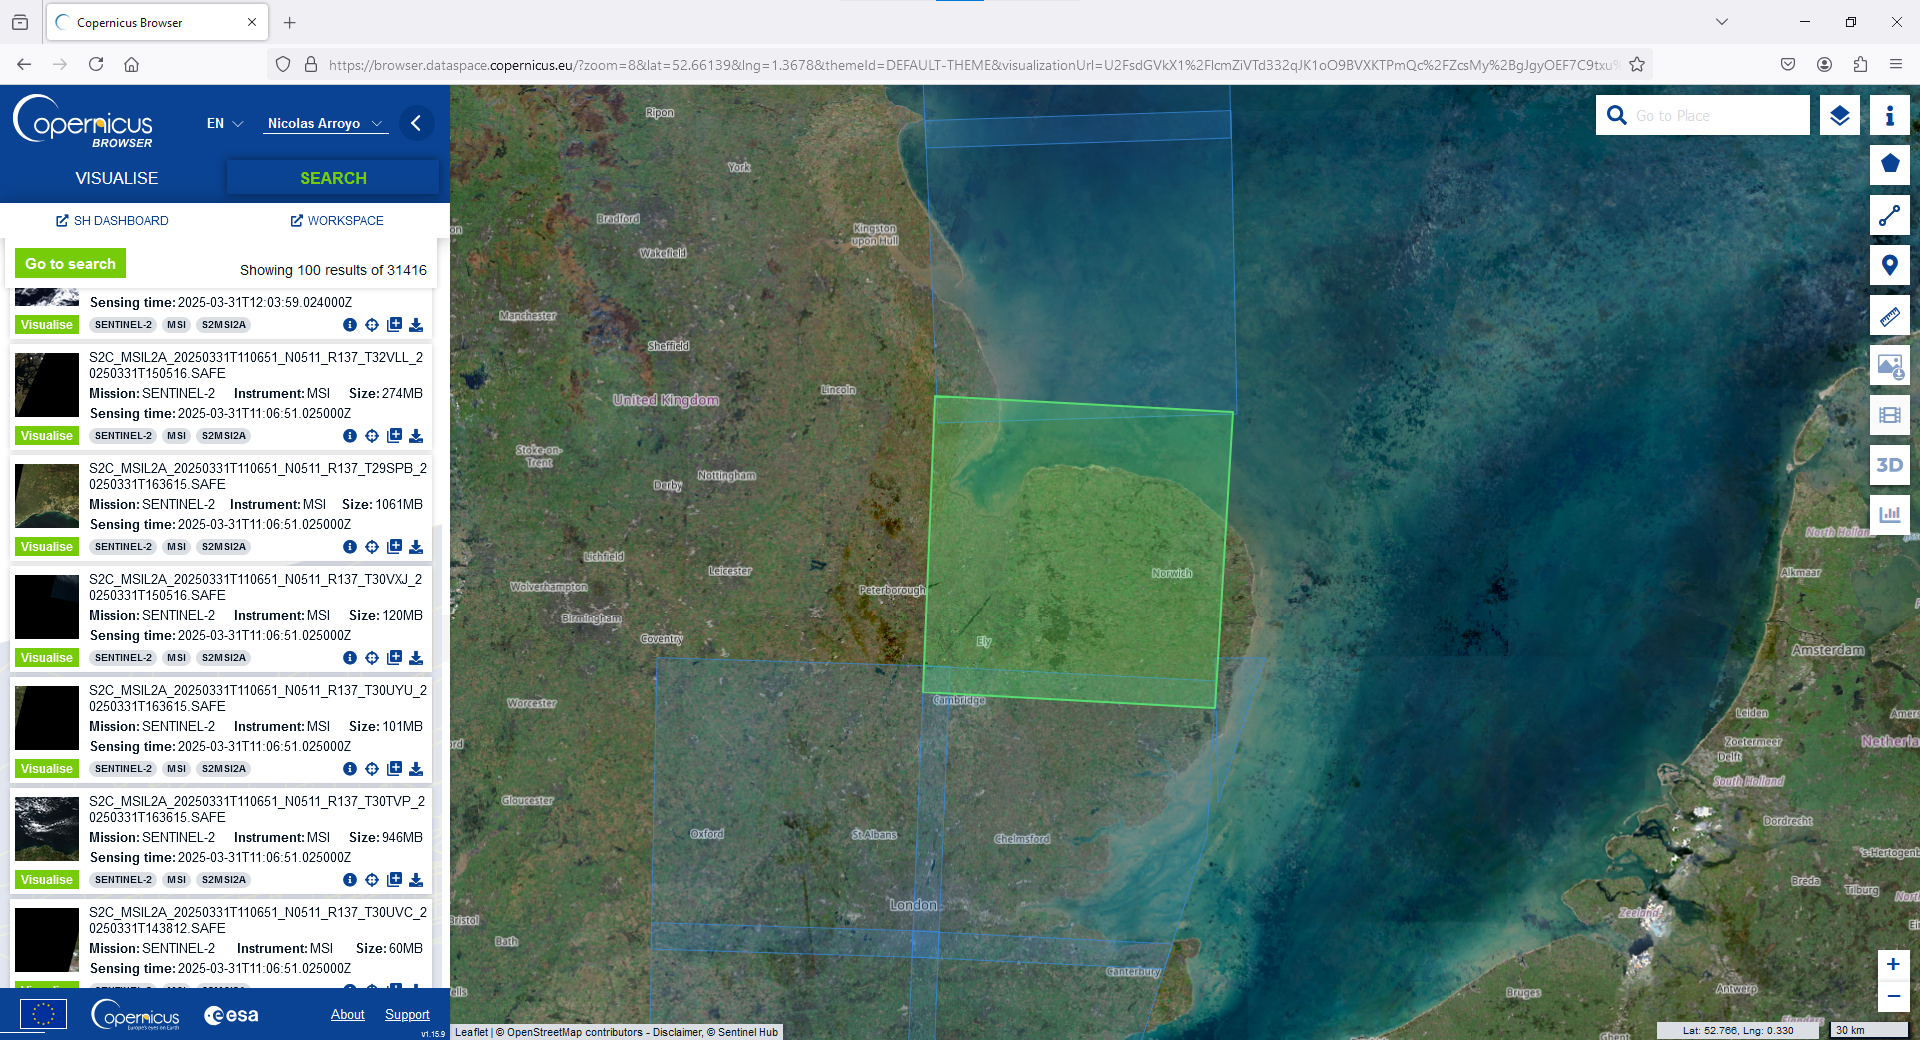
\includegraphics[width=0.5\linewidth]{contents/figures/ME copernicus example chunk.jpg}
    \caption{Copernicus browser image example}
    \label{fig:ME copernicus image example}
\end{figure}
The Copernicus browser will take some time to load the images. After you can see the image names on the left-hand side of the screen, select one where the land is clearly visible in the East Midlands area, as demonstrated in figure \ref{fig:ME copernicus image example}. To download this image, simply press the download button as demonstrated in figure \ref{fig:ME copernicus download example} and wait for the file to download completely. Note: satellite image files are usually very large (around 1 GB in size). The files are packaged in \verb|.zip| folders on Windows which have to be extracted. Further image processing and data generation will increase the required storage available, so ensure you have at least 5 GB available on disk, or use online storage solutions. This is discouraged as there have been incidents of files being deleted automatically by services like OneDrive. 

\begin{figure}[H]
    \centering
    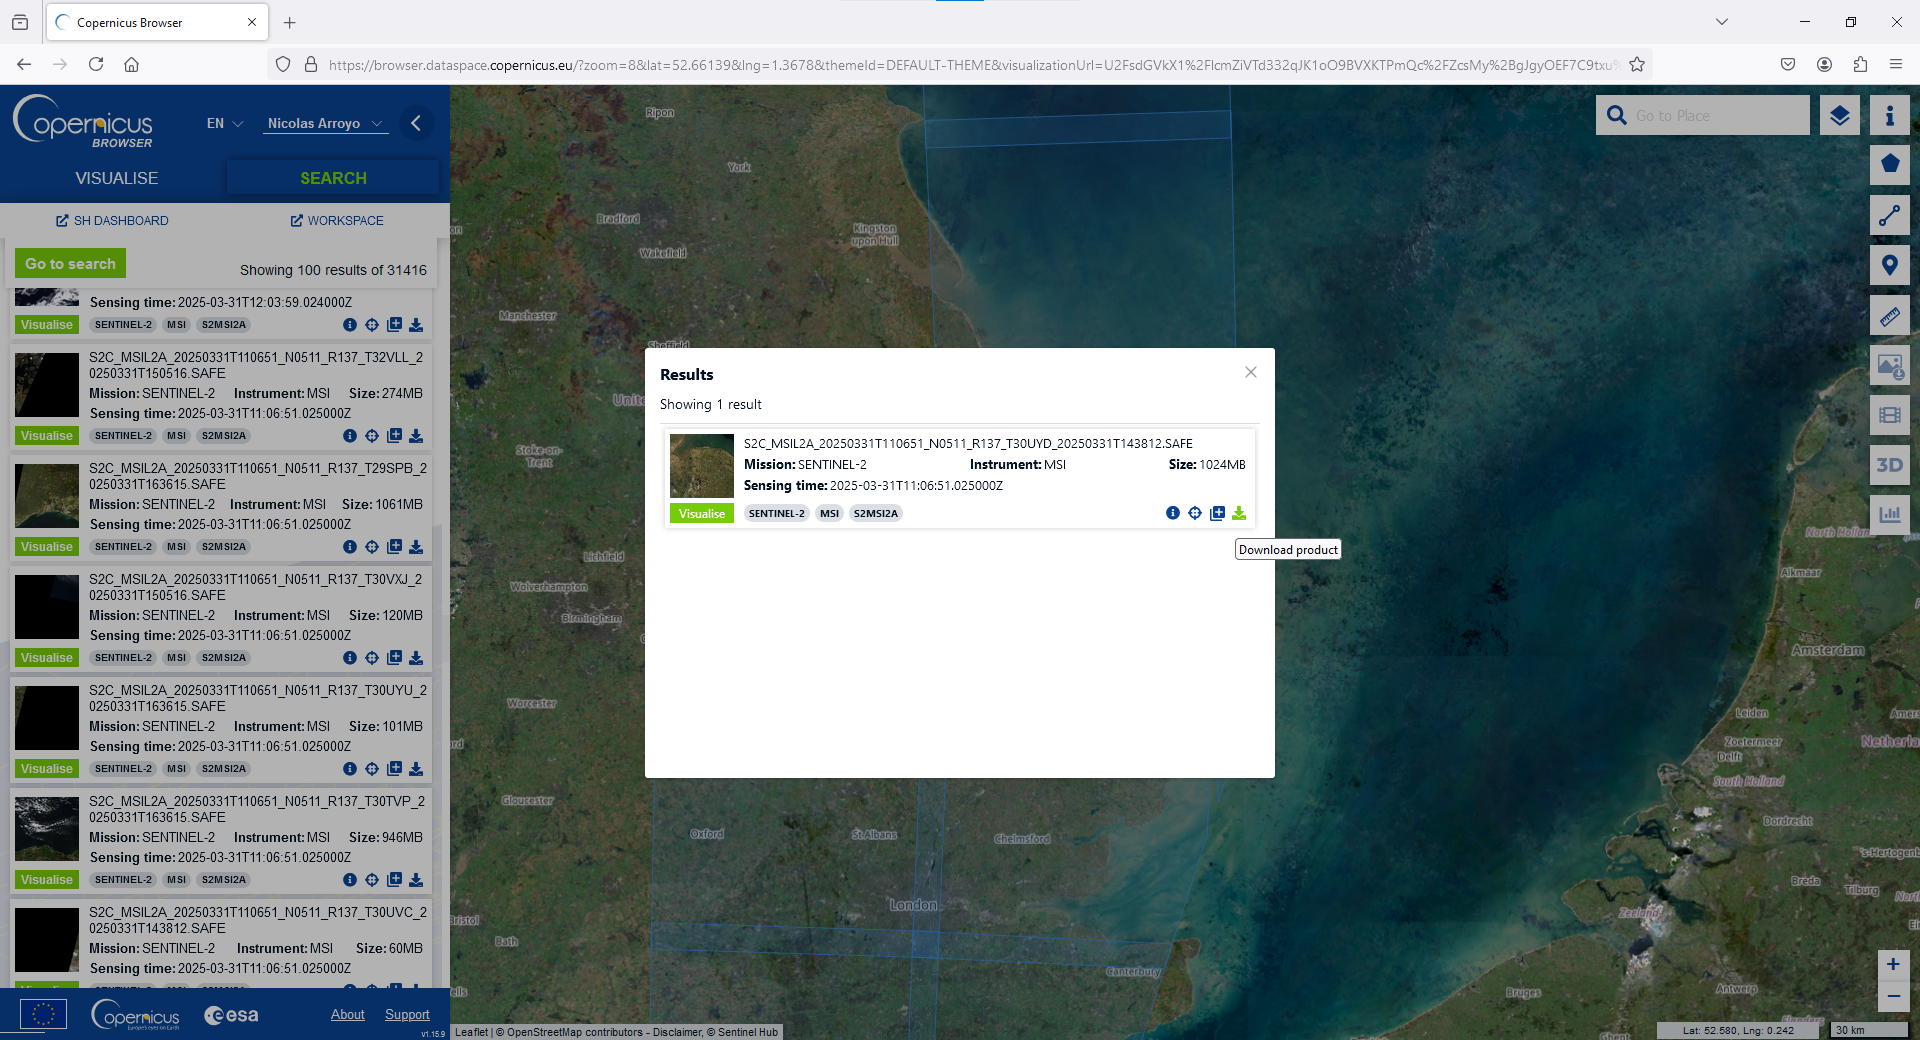
\includegraphics[width=0.5\linewidth]{contents/figures/ME copernicus download example.jpg}
    \caption{Copernicus browser download example}
    \label{fig:ME copernicus download example}
\end{figure}
Once the image folder has downloaded completely, extract the zip file to a known location, preferably close to the root of your drive to prevent \verb|maximum path length| errors. This error occurs when Python or the operating system tries to access a file but the path to that file is too long (above 250 characters). This can be disabled when installing Python, but to avoid any potential problems, it is generally good practice and strongly recommended to store this folder close to the root. 

For example:

"\verb|C:\Users\abcde\Sen2|" 

as opposed to something like 

"\verb|C:\Users\abcde\Documents\Satellite Image Downloads\Sentinel 2|"

\begin{figure}[H]
    \centering
    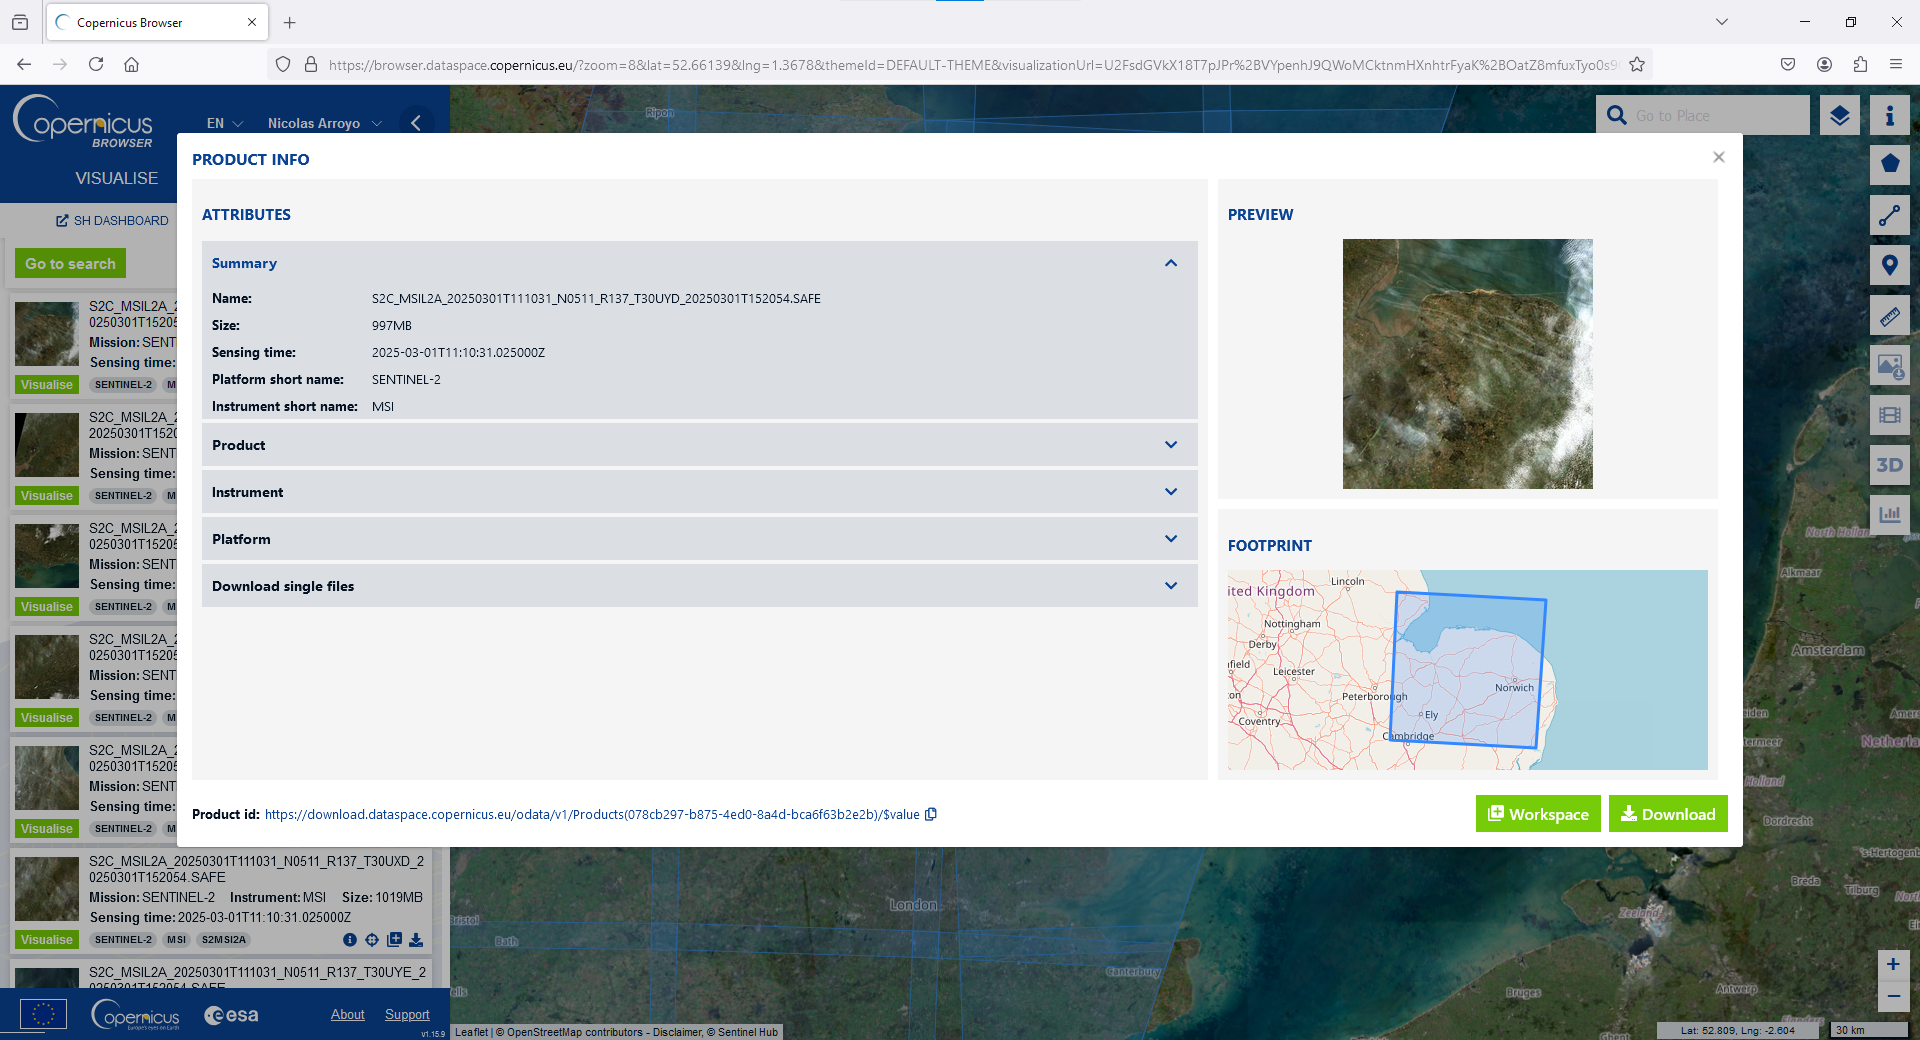
\includegraphics[width=0.5\linewidth]{contents/figures/ME copernicus exact chunk.jpg}
    \caption{Copernicus browser exact development image used}
    \label{fig:ME copernicus exact image}
\end{figure}
The actual image used for initial program development is the one shown in figure \ref{fig:ME copernicus exact image}. The name of this image is as follows: 

\verb|S2C_MSIL2A_20250301T111031_N0511_R137_T31UCU_20250301T152054.SAFE|

For all following file naming explanation or referencing, this is the image name that is being used. 

\subsection{Sentinel File Naming Convention}
Each satellite image folder from the Sentinel satellites follows the same naming convention. This simplifies file searching and enables the automation developed with NALIRA. All the main, important details about a given satellite image is stored in its folder name, and anything that is seen as too granular to include in the name is stored in various meta-data files within the folder. For this study, none of the meta-data information is necessary, so it is important to first explain the meaning of the image folder name. 

Every section of information is split up with underscores ("\verb|_|"), so in total there are seven main sections. We will use the exact image folder that was used for program development in this study to identify these sections. All of this information is given by \cite{copernicus_2025}

\verb|S2C_MSIL2A_20250301T111031_N0511_R137_T31UCU_20250301T152054.SAFE|

\subsubsection{S2C}
The first section is simply the name of the satellite. In this case, "S2C" stands for "Sentinel 2 C". This bit could also be "S2A" or "S2B" if using Sentinel 2 A or Sentinel 2 B. 

\subsubsection{MSIL2A}
This sections contains two pieces of information: the first three characters, "MSI" are the abbreviation of the instrument used (MSI = Multi-Spectral Instrument) and the last three characters are the product level (L2A = Product Level 2, meaning that some post-processing has been applied). 

\subsubsection{20250301T111031}
This is the "datatake start sensing" time. It is split up into the format: 

\verb|YYYYMMDDTHHMMSS|, where \verb|YYYYMMDD| is the year, month, and day, and \verb|HHMMSS| is the hour, minute, and second of the day that the sensor started imaging to produce this data. The \verb|T| character is used to separate the data and time. 

\subsubsection{N0511}
This is the "Processing Baseline Number", which gives more information about the processing level. 

\subsubsection{R137}
This is the "Relative Orbit Number", which can range from \verb|001| to \verb|143| because 143 is the number of full orbits that the satellites make before completing a full cycle. 

\subsubsection{T31UCU}
This is the "tile number field", which essentially describes the 110 km x 110 km area being imaged. There are enough tiles to cover everywhere that a Sentinel 2 satellite could take an image of, so we can use this section to find where on Earth the image is covering. This information can then be used to conduct image compositing, which, although not implemented for this project, is a possible area of future development. 

\subsubsection{20250301T152054.SAFE}
Finally, this section is the "Product Discriminator". It follows the same format as the datatake start sensing time, however it can be slightly earlier or later than the start time depending on which product it is describing. 

The \verb|.SAFE| suffix is the "Standard Archive Format for Europe". 

\subsubsection{Sub-folders and files}
The image sub-folder contained in the main image folder may have a different format to each other, however, the sub-folder is always the only item in that level of the directory, so it is relatively simple to search the level and find the sub-folder. The image files themselves all follow a cohesive format. 

If we are trying to access a \verb|10m| resolution \verb|green| band image, we first need to recall which band on Sentinel 2 senses the green wavelength. In table \ref{tab:LR s2 band wavelengths and resolutions}, we can see that the green band is number \verb|3|. We can combine the tile number field, the datatake start sensing time, the band number, preceded by the letter \verb|B| and a \verb|0| if it is a single digit band number, and the resolution. At the end, we have to place the image file format, which is \verb|JPEG2000| for Sentinel 2 images. This is a lossless version of the \verb|jpg| format, and it means that all images are stored with the \verb|.jp2| file extension. The native Windows photo viewer is not capable of opening these images, so it may be helpful to install an image manipulation program like \verb|GIMP| to view these images, although it is not necessary for the processes outlined here. This yields the following file name: 

\verb|T31UCU_20250301T111031_B03_10m.jp2|

This image file is stored within subdirectories of the main folder, and this will be covered in an upcoming section. 

\section{IPDMP System Overview}
The Individual Project Data-to-Model Pipeline (IPDMP) comprises three core Python scripts designed for the classification of small water reservoirs using Sentinel 2 satellite imagery. The overall process involves data generation and labelling (NALIRA), model training (KRISP trainer), and model deployment for prediction (KRISP).

For this study, the Normalised Difference Water Index (NDWI) is selected as the primary spectral index for data labelling and model training/validation due to its ability to leverage Sentinel-2's high-resolution bands (Green and NIR). While other indices like MNDWI, AWEI-SH, and AWEI-NSH are calculated in NALIRA to aid manual labelling by providing multiple visual inputs, the machine learning model focuses on NDWI-derived data.

\begin{lstlisting}[language=Python, caption=Calculation of Water Detection Indices]
np.seterr(divide="ignore", invalid="ignore")
ndwi = ((green - nir) / (green + nir))
mndwi = ((green - swir1) / (green + swir1))
awei_sh = (green + 2.5 * blue - 1.5 * (nir + swir1) - 0.25 * swir2)
awei_nsh = (4 * (green - swir1) - (0.25 * nir + 2.75 * swir2))
\end{lstlisting}

Cloud masking employs a basic numerical threshold approach. Pixels in the Sentinel-2 cloud probability band (\verb|MSK_CLDPRB|) with a likelihood greater than 50\% are masked (set to NaN or zero) in the band images before index calculation. This simple method is deemed sufficient due to the selection of imagery from a period with known low cloud cover (March 2025). For applications in cloudier periods, more advanced masking techniques (e.g., FMask) and image compositing would be necessary.

A custom Keras-based Convolutional Neural Network (CNN) model, adapted from a TensorFlow tutorial, is used for classification. This approach offers flexibility and aims for good generalisation on the study area. The model is trained to classify image segments into 'reservoirs', 'water bodies' (non-reservoir), or 'land'. The KRISP script then deploys this trained model, applying it iteratively across small image chunks ('mini-chunks') derived from the larger satellite scene, effectively acting as an object detection mechanism for water reservoirs.

\subsection{Helper Functions}
To improve code readability, each of the programs discussed below make use of helper functions. This also improves the efficiency of the code as fewer variables need to be stored in memory and each file is itself smaller

\section{Objective 2: Data Generation (NALIRA)}
The second step is to generate training data. Rather than lengthy and laborious manual labelling, this study develops the Navigable Automated Labelling Interface for Regions of Attention, abbreviated to NALIRA. 

This Python program ingests a Sentinel 2 satellite image, extracts the necessary bands for index calculation, conducts cloud masking, performs index calculations, optionally displays the plots of the indices calculated, manipulates a "True Colour Image" (TCI) found in the Sentinel 2 data folder, and separates the images and index plots into a user-defined number of "chunks". This is done to make data labelling easier for the user as it allows them to split the process up into shorter period of data labelling. So far, the entire process described is entirely automated to offload user intervention onto robust checks and verifications done automatically by the program. 

After the images are split into chunks, the user is iteratively prompted with each chunk and they must enter the number of reservoirs and water bodies in the chunk. If they input one or more of either class, a Graphical User Interface (GUI) is produced for the user to identify (label) those reservoirs or water bodies which are named and saved as regions of interest (ROIs). These "chunk-wise" coordinates are saved to a "comma-separated values" (CSV) format file. 

This file is rigorously checked for file and data validity before the data labelling process even begins, and if any error or inconsistency is found, the user is prompted to fix the error before being allowed to proceed. The file is also checked continuously with every successive chunk to ensure minimal chance of failure, which could result in the loss of a large amount of training data. 

During data labelling, the user is also able to take a break and the progress is automatically saved on disk, or return to any previous chunk examined to view it again and overwrite their entry, introducing the navigable element of NALIRA. Once data labelling is either complete for the entire image or the user has decided to take a break, the automation is resumed and the chunk-wise coordinates are used to individually isolate each reservoir and water body in an image $\frac{1}{25}$ the size of the chunk and that image is saved as training data for both NDWI and TCI. Similar images are saved for non-water land by selecting the top left corner of each chunk with no reservoir or water body. 

\subsection{NALIRA Code Walk-through}


\section{Objective 3: Model Training (KRISP Trainer)}
This script trains the Keras CNN model using the segmented image data generated by NALIRA. This is the script that was adapted from an existing image classification tutorial created to classify images of different types of flowers \citep{imageclassification_2024}. 

\subsection{Changes from Flower Classification}
Originally, the flower classification tutorial had several steps which were not directly applicable to this study, as can be seen in figure \ref{fig:ME outline OG flower classification}. 

\begin{figure}
    \centering
    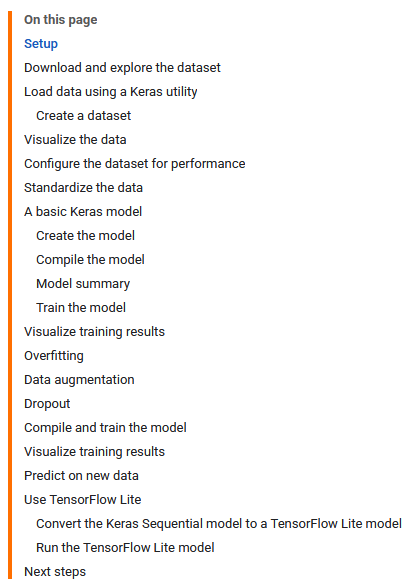
\includegraphics[width=0.5\linewidth]{contents/figures/ME outline of flower classification.jpg}
    \caption{Table of Contents for the original flower classification tutorial \citep{imageclassification_2024}}
    \label{fig:ME outline OG flower classification}
\end{figure}

Some of the steps up to \verb|A basic Keras Model| are necessary for proper data handling, although they had to be adapted to function with the specific paths used in KRISP Trainer. Most of these initial steps, however, are not necessary for the function of KRISP Trainer, such as \verb|Visualize the data| which simply chooses an image from the dataset and displays it in the console. These steps were removed for KRISP Trainer, which is solely concerned with handling data and training the model. 

The basic Keras model created in the tutorial is used as a way of showing the common pitfalls of machine learning, specifically overfitting, and the two techniques used to mitigate this problem, data augmentation and dropout. To avoid training unnecessary models, the training of the basic Keras model with no mitigations against overfitting was removed altogether, but the strategies of data augmentation and dropout were both included in the training of the final model. 

The steps of \verb|Compile and train the model|, \verb|Visualize training results|, and \verb|Predict on new data|, were all preserved and adjusted for KRISP Trainer. Although visualising training results is not explicitly necessary for model training, it is helpful for identifying the ideal duration of training and for spotting the inflection point as the model suffers from overfitting. 

\begin{figure}
    \centering
    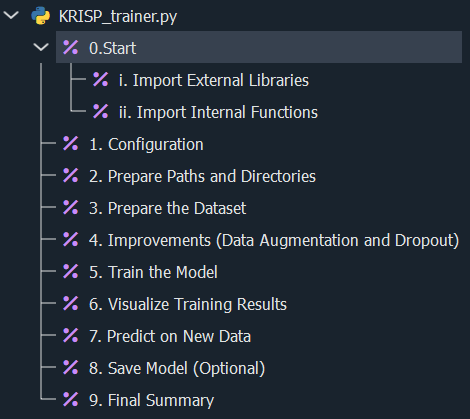
\includegraphics[width=0.5\linewidth]{contents/figures/ME KRISP trainer outline.jpg}
    \caption{Table of Contents for KRISP Trainer \citep{imageclassification_2024}}
    \label{fig:ME outline krisp trainer}
\end{figure}

As can be seen from figure \ref{fig:ME outline krisp trainer}, the contents of KRISP Trainer are significantly reduced to the ones of the original flower image classification tutorial. Given that the tutorial is designed to explain each step in detail, the steps that were deemed "unnecessary" are in reality very useful in understanding the strategies behind the training of a Keras model. However, efficiency and performance are a priority throughout this project, so KRISP Trainer keeps only the essentials from the flower classification tutorial and the rest is reworked for the purposes of this particular study. 

\subsection{KRISP Trainer Code Walk-through}


\section{Objective 4: Model Deployment (KRISP)}
This script deploys the trained Keras model (saved by \verb|KRISP_trainer|) to classify mini-chunks generated from a larger Sentinel-2 scene. While the KRISP program makes predictions over a given number of chunks, the KRISP-Yield program (KRISP-Y) was developed to yield the data (predictions) made by KRISP and to save everything to a CSV file. 

\subsection{KRISP Code Walk-through}

\subsection{KRISP-Y Code Walk-through}

\section{Technical Challenges}
\subsubsection{Identifying water}
One of the main challenges in this research will be the differentiation between water reservoirs from land areas, or other bodies of water. Below is a screenshot taken from Google Maps showing a farm in east England with a water reservoir in the middle, some tree cover nearby, and a house. 

\begin{figure}[H]
\centering
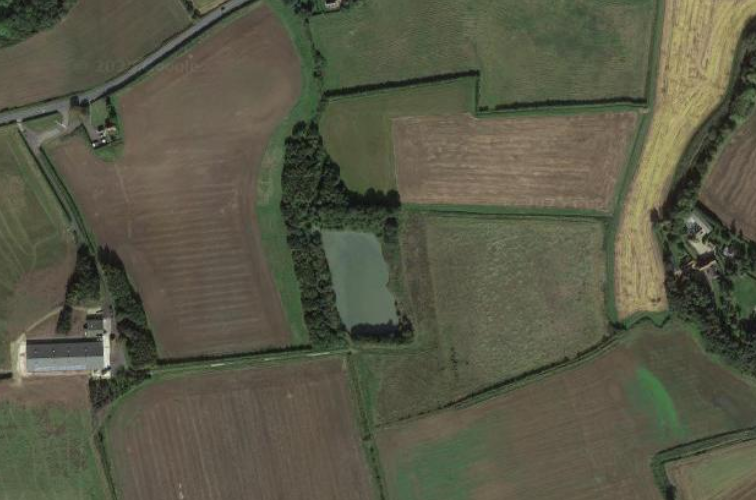
\includegraphics[width=0.4\textwidth]{contents/figures/gmaps screenshot.jpg}
\caption{Google Maps screenshot showing a water reservoir near trees}
\label{fig:NISH}
\end{figure}

In this example, a human could easily identify that the upper right side of this image shows trees, and the lower left side shows a river with a nearby water reservoir. However, a computer algorithm may find this differentiation more difficult, as relying solely on colours may lead it to the conclusion that both sides of the image contain a water reservoir. Instead, more complex techniques must be adopted that allow the computer to determine the shape, surrounding area, and other contextual information about the water reservoir. For this reason, one of the goals of this project is also to determine what the most valuable metrics are, from a satellite imagery perspective, for identifying water reservoirs. A further challenge will then be implementing these metrics and training a machine learning algorithm to make use of them to classify large areas of land. 

\subsubsection{Cloud Contamination}
Satellite imagery can come in many different levels of quality, and one of the main problems that have to be mitigated for is potential cloud cover. Clouds can partially or completely obscure important features on land or they can 'trick' a program into predicting a water feature instead of a cloud or the shadow of a cloud. As mentioned before, the time period for this study was specifically selected to avoid this problem entirely, however for the cases where clouds still cover part of the image, rudimentary cloud masking has been implemented, and will be discussed in further detail in upcoming sections. 

\subsubsection{Machine Learning Development}
There are also technical challenges that come with machine learning. Although resources for learning about this topic have improved in the past few years, there is still a steep learning gradient, particularly for one with little background in computer science. For this reason, the researcher has diligently documented progress on software development in this project with a public code repository which can be found linked in Appendix B. 

\section{Online Code Repository (GitHub)}
See appendix B
